\chapter{Neural Network Noise Suppression}\label{NeuralNetworkNoiseSuppression}
In this section the Machine learning approach will be explained together with the signal processing needed for it.
This method will be used to suppress the noise from the signal, keeping the speech as clean as possible.
\section{Signal Processing}
\label{SignalProcessing}
A sound wave at its most basic form is described as a vibration that propagates in a medium as gas, liquid or solid as an audible fluctuation in pressure. A transducer, as a microphone has a diaphragm that vibrates according to those fluctuations. In this way the amplitude, the power of pressure, can be recorded. Another property of of sound wave is the frequency, which is the variation of the amplitude over time, which can be easily calculated from a two dimensional plot, with the two axis being the amplitude and the time, looking at the number of occurrences of a cycle in a unit of time.
\subsection{signal preprocessing}
As sound is an analog signal, for recording that signal it will have to be sampled. Depending on the sampling rate, the sound signal can have varying degree of quality, human ears are most the most sensitive in the range of 100 to 3000 Hz which are also called the fundamental frequencies. But human voice also has harmonics which are in the range of 900 Hz to 17 KHz.
According to the Nyquist rate of signal processing, the sample rate should be at least double the frequency of the signal in order to avoid aliasing. 
\todo[inline]{Fits in development or introduction?}
\todo{link the nr of picture in text}
\newpage
\begin{figure}[htp]
	\centering
	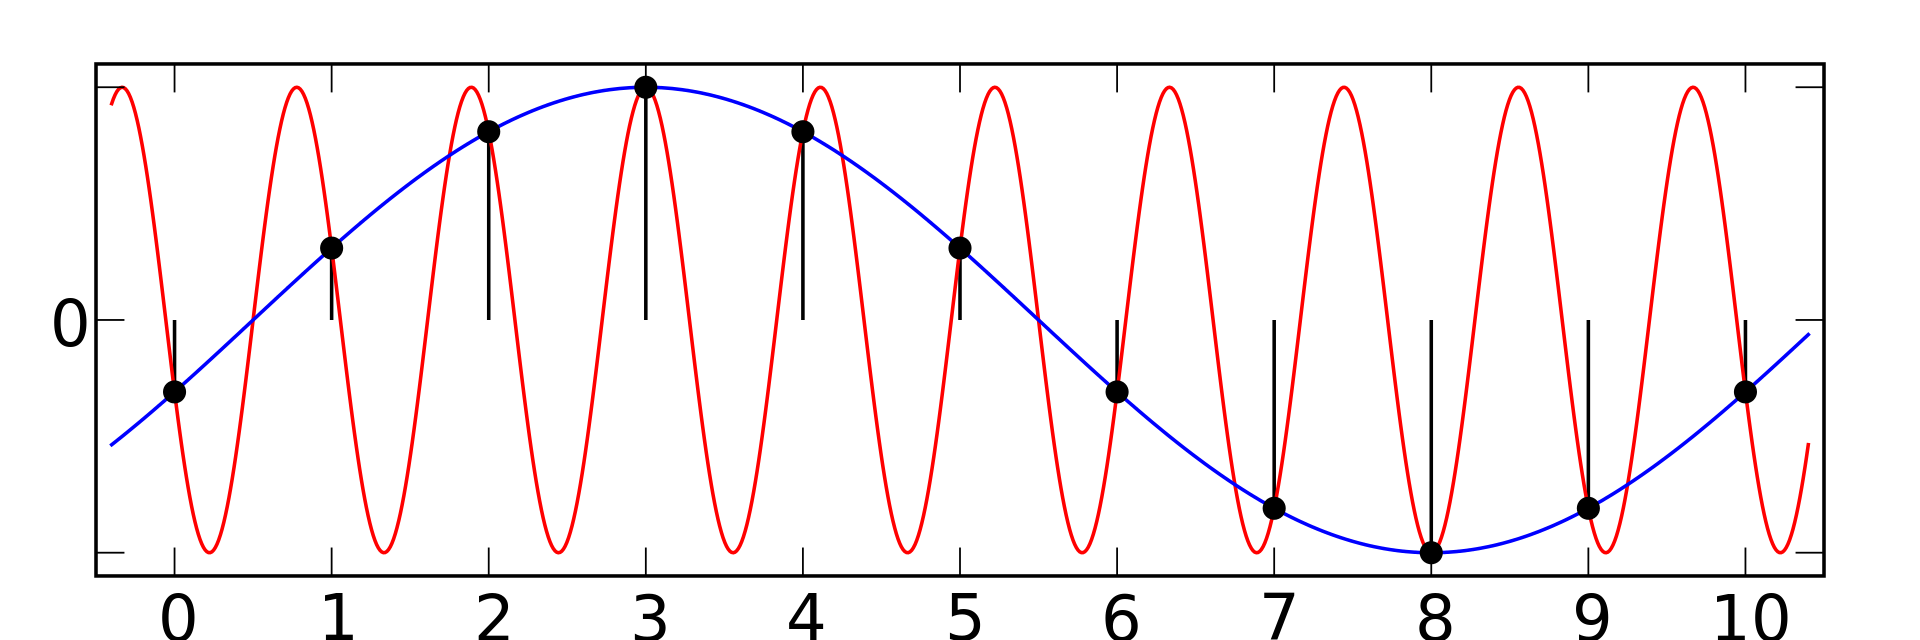
\includegraphics[width=1\textwidth]{Illustrations/AliasingSines.png}
	\caption{Consequences of different sampling rates}
	\label{fig:AliasingSines}
\end{figure}

As we can see in figure \todo{add here nr} if the sampling rate is too small, the signal will be aliased and will get a wrong representation of the signal.

\subsection{Fourier Transform}
As useful as the amplitude might be, for a closer inspection of a signal it is not enough to differentiate human speech from different sound sources. Any sound signal can be recreated from a combination of sinusoidal signals at different frequencies.  For that reason the Fourier Transform can be used to decompose the sound in multiple frequencies. By transforming the signal from the time domain to the frequency domain we can get a lot more information about a specific signal. By plotting these, we will get the amplitude of each frequency over the whole signal.

\begin{figure}[htp]
	\centering
	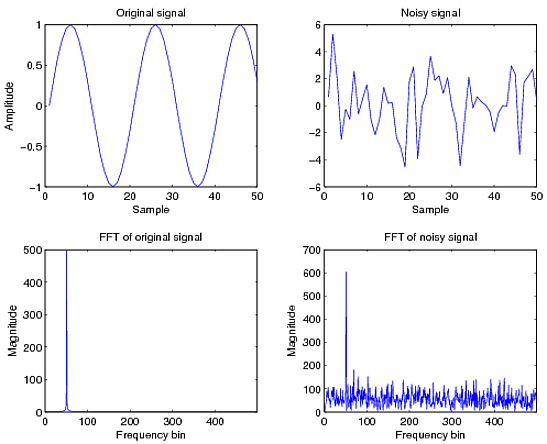
\includegraphics[width=0.6\textwidth]{Illustrations/fftSignals.png}
	\caption{FFT representation of a sine wave and a noisy one}
	\label{fig:fftSignal}
\end{figure}
\newpage
As we can see in figure \todo{add nr for picture} besides being able to differentiate between different sound sources, especially clean speech, as it was said in a different sections, we know the frequencies in which human voice is so we can see it easier in a frequency domain representation , we can identify noise easier too.

\subsection{Spectrogram of a signal}
Except for perfect examples, just a Fourier transform plot will not be that useful as some sound sources can be only in a part of the full sample and by viewing the plot over the whole sample it will not be accurate enough for filtering. For this reason a spectrogram can be used, which instead of taking the Fourier transform over the whole sound sample, it will make multiple ones over 0.25 second frames. By doing this we can get 3D plot, where we can have the X axis for time or samples, Y axis for the frequencies and color for the amplitude. By doing this a really clear representation of the signal can be made from which multiple aspects of the signal can be seen and used.

\todo{ADD picture of spectrogram with speech from matlab}

\subsection{Mel-frequency cepstrum}
A Mel-frequency cepstrum is made out of a multitude of Mel-Frequency cepstral coefficients(MFCCs). Those are taken from a cepstral representation of the audio sample(or a spectrum of a spectrum).
This can be really useful especially for speech identification as the frequency bands are spaced equally on the Mel scale instead of linearly spaced frequency used in a normal cepstrum. The mel scale is more useful for this case as it better approximates how humans actually perceive sound.
\todo{maybe photo, most probably photo} 


Besides this, instead of using the full cepstrum, only 24 bands can be used, by using the Bark scale instead.
The bark scale is psychoacoustical scale that represents the first 24 critical bands of hearing. This can easily be made as mel scale and Bark scale are proportional to each other as 1 Bark is approximately equal to 100 mels.\todo{add reference}
By doing this, memory and processing power can be saved by using only 24 bands instead of thousands.
\begin{figure}[htp]
	\centering
	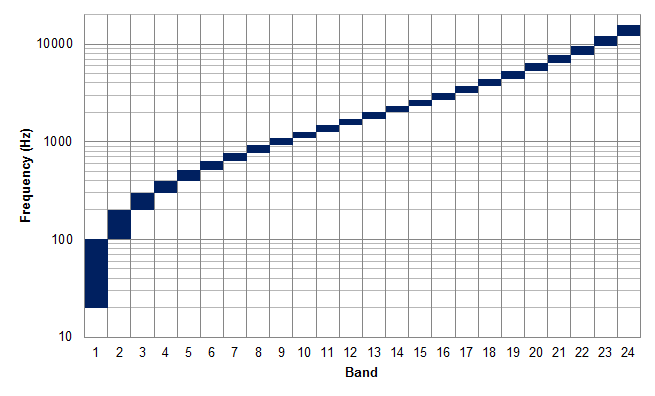
\includegraphics[width=1\textwidth]{Illustrations/Bark_scale.png}
	\caption{The 24 bands of the Bark Scale}
	\label{fig:BarkScale}
\end{figure}
\newpage
\section{Artificial Neural Network Theory}

An Artificial Neural Network is a a machine learning technique or computing system that slightly resembles a brain and its neuronal connections. Being programmed without specific rules, an ANN system has one or more layers of artificial neurons with specific weights associated to each one of them. By giving the system multiple input sequences, it will \"train\" itself by adjusting the weights to have an output prediction that will resemble the wanted output as much as possible.

\subsection{Artificial  Neurons}

An artificial neuron is an elementary unit in an artificial neural network. As being inspired by biological neurons, their purpose is to simulate the different function that they have:
\begin{itemize}
\item Gathering all the inputs
\item Multiplying with their each individual weight
\item Adding all the weighted inputs
\item The sum will be passed to the activation function
\item Outputting the result
\end{itemize}

\begin{figure}[htp]
	\centering
	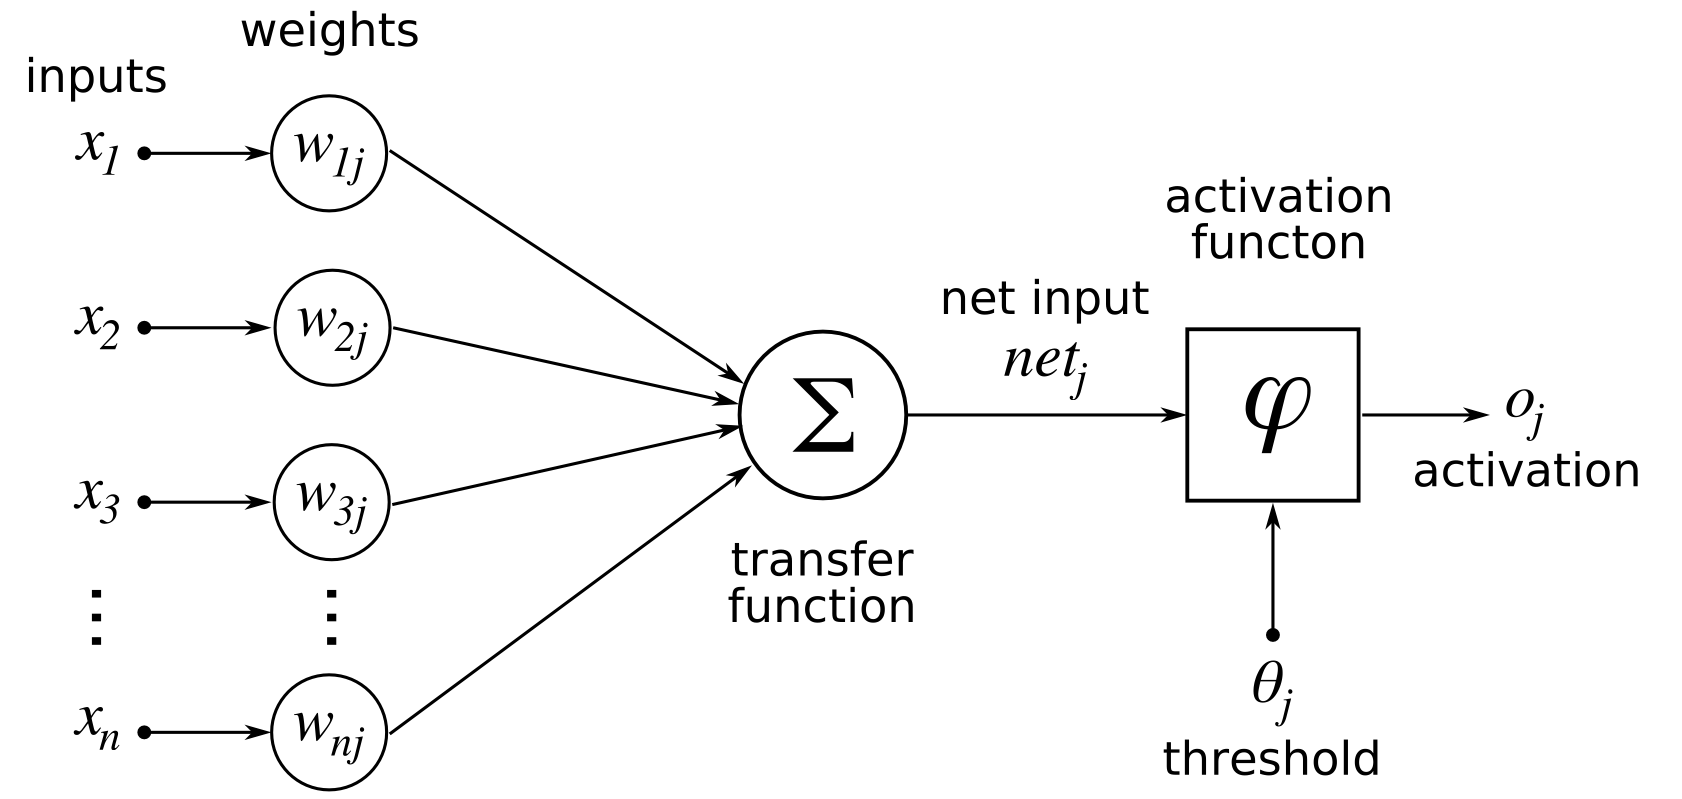
\includegraphics[width=1\textwidth]{Illustrations/artificialneuron.png}
	\caption{Example of an Artificial Neuron}
	\label{fig:ArtificialNeuron}
\end{figure}

In figure \todo{add nr of figure}, representing an artificial neuron, all those functions can be seen. The neurons will be received, multiplied by a vector of weights, added together and sent to the activation function which will then give the output of the artificial neuron.

\subsection{Activation Functions}

As stated in the last section, each neuron will have an activation function. Being biological inspired, it usually represents the rate of action potential in the cell, depending on the range and the case, this can be from 0 to 1 or from -1 to 1. In the range of 0 to 1, which resemble the biological neuron more, this can be seen as the neuron firing or not.

Two of the most used activation function are:
The sigmoid Function:

\begin{itemize}
\item The sigmoid Logistic Function: Which maps the input from 0 to 1.This can be really useful where neurons have to predict the probability as the output.
\begin{equation}
 \sigma(z) = \frac{1}{1+e^{-z}}
\end{equation}

\item Hyperbolic tangent function: Which maps the input from -1 to 1. This can be used when the classification between two classes is needed.
\begin{equation}
 \phi(z) = tanh(z)= \frac{2}{1+e^{-2x}}-1
\end{equation}

\end{itemize}

\begin{figure}[htp]
	\centering
	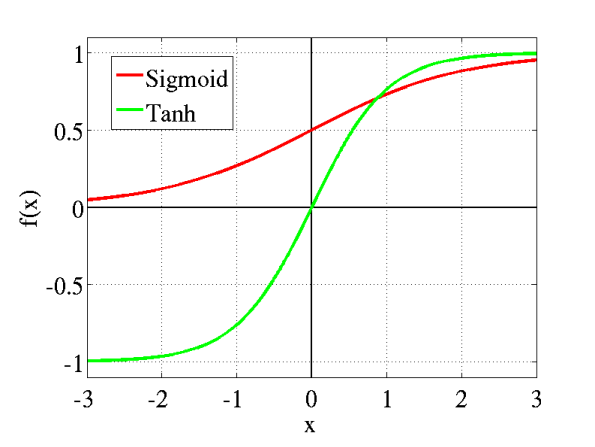
\includegraphics[width=0.5\textwidth]{Illustrations/sigmoidandtangent.jpeg}
	\caption{Both sigmoid and tangent functions exemplified}
	\label{fig:SigmoidAndTangent}
\end{figure}

\subsection{Types of Artificial Neural Networks}

\subsubsection{Feed-Forward Networks}

The feed-forward neural network is one the first methods invented and one of the simplest. As the name suggests, the information moves only forward from the input, through the hidden layers is it has any, to the output. All neurons are directly connected to the neurons from the next layer, they have no cycles or loops like other other neural networks that are going to be presented.

Different types exists, as single layer perceptron, which have the inputs being fed directly in the output layer using a series of weights. Multi-layer perceptron is another one, which,compared with the single layer perceptron, has one or more hidden layers of neurons.
In most cases a sigmoid activation function is going to be used for those types of neurons as they are usually used for classification purposes.In other types like Convolution neural networks,which are composed of one or more convolutional layers, have fully connected layers, meaning that all the lengths of the output vector will be equal with the input one.

\subsubsection{Recurrent Neural Networks}

Recurrent Neural Networks are is an artificial neural network model which uses sequential information. In other models, like feed-forward networks, all the input and outputs are independent of each other, meaning that one series of inputs cannot affect the result of others.
This can be really useful in some cases like translation, speech recognition, sound optimization, text prediction, where giving an output based on past iterations can be more precise and easier or even completely necessary in some cases.


\subsubsection{Gated Recurrent Unit Networks} 

Gated Recurrent Unit Networks 

